The adaptive data analysis designed for identifying  properties for unknown populations / distributions 
through data samples is widely 
used in research and industrial areas.
% , including machine learning areas, etc.. 
When generalizing the analysis result from data samples to the unknown populations, 
the generalization error is the key issue on which researchers are focusing to reduce.
% Since An 
Especially in the adaptive data analysis,
% the
%  can be seen as 
which is a process composed of 
multiple queries interrogating some data
%  in the analysis are , 
% where 
the choice of which query to run next may rely on the results of previous queries. 
The generalization error is propagated through the reliance between the choices of queries.
In this sense, the \emph{adaptivity} rounds (i.e., how many queries are relied on others) in the analysis plays a key role in reducing the generalization error.
Below I introduce in detail the significance and limitation of this \emph{adaptivity} quantity.
\paragraph{Adaptive Data Analysis Limitation}
\label{sec:intro-exelimitation}
Consider a dataset $X$ consisting of $n$ independent samples from some unknown population $\dist$. How can I ensure that the conclusions are drawn from $X$ \emph{generalize} to the population $\dist$? Despite decades of research in statistics and machine learning on methods for ensuring generalization, there is an increased recognition that many scientific findings generalize poorly (e.g. 
\cite{Ioannidis05,GelmanL13}
). While there are many reasons a conclusion might fail to generalize, one that is receiving increasing attention is \emph{adaptivity}, which occurs when the choice of method for analyzing the dataset depends on previous interactions with the same dataset~\cite{GelmanL13}.

 Adaptivity can arise from many common practices, such as exploratory data analysis, using the same data set for feature selection and regression, and the re-use of datasets across research projects. Unfortunately, adaptivity invalidates traditional methods for ensuring generalization and statistical validity, which assume that the method is selected independently of the data. The misinterpretation of adaptively selected results has even been blamed for a ``statistical crisis'' in empirical science~\cite{GelmanL13}.
% ~\cite{GelmanL13}.

A line of work initiated by \cite{DworkFHPRR15}, \cite{HardtU14} posed the question: 
Can I design \emph{general-purpose} methods that ensure generalization in the presence of adaptivity, together with guarantees on their accuracy? 
The idea that has emerged in these works is to use randomization to help ensure generalization. 
Specifically, these works have proposed to mediate the access of an adaptive data analysis to the data utilizing queries from some pre-determined family (I will consider here a specific family of queries often called "statistical" or "linear" queries) that are sent to a 
\emph{mechanism} which uses some randomized process to guarantee that the result of the query does not depend too much on the specific
sampled dataset. 
%
\begin{figure}
 \centering
 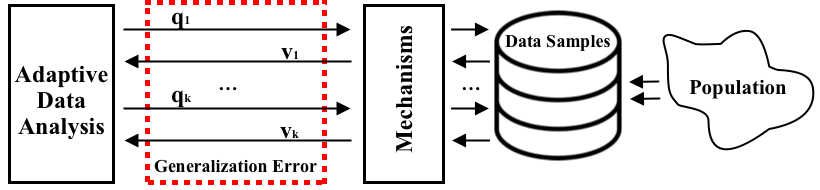
\includegraphics[width=0.7\columnwidth]{figures/data_analysis_model.png}
 \caption{Overview of our Adaptive Data Analysis model.}
 \label{fig:adaptivity-model-overview}
\vspace{-0.5cm}
\end{figure}
This guarantees that the result of the queries generalizes well. 
This approach is described in Figure~\ref{fig:adaptivity-model-overview}, where
I have a population that I am interested in studying, and a dataset containing individual samples from this population. The adaptive data analysis I am interested in running has access to the dataset through queries of some pre-determined family (e.g., statistical or linear queries) mediated by a mechanism. 
This mechanism uses randomization to reduce the generalization error of the queries issued to the data.
This line of work has identified many new algorithmic techniques for ensuring generalization in adaptive data analysis, leading to algorithms with greater statistical power than all previous approaches. 
Common methods proposed by these works include the addition of noise to the result of a query, data splitting, etc. 
Moreover, these works have also identified problematic strategies for adaptive analysis, showing limitations on the statistical power one can hope to achieve. 
Subsequent works have then further extended the methods and techniques in this approach and further extended the theoretical underpinning of this approach, 
e.g.~\cite{dwork2015reusable,dwork2015generalization,BassilyNSSSU16,UllmanSNSS18,FeldmanS17,jung2019new,SteinkeZ20,RogersRSSTW20}.
%

A key development in this line of work is that the best method for ensuring generalization in an adaptive data analysis depends to a large extent on the number of \emph{rounds of adaptivity}, the depth of the chain of queries. 
As an informal example, the program $x \leftarrow \query_1(D);y \leftarrow \query_2(D,x);z \leftarrow \query_3(D,y)$ has three rounds of adaptivity, since $\query_2$ depends on $D$ not only directly because it is one of its input but also via the result of $\query_1$, 
which is also run on $D$, and similarly, $\query_3$ depends on $D$ directly but also via the result of $\query_2$, which in turn depends on the result of $\query_1$. 
The works I discussed above showed that not only does the analysis of the generalization error depend on the number of rounds, 
but knowing the number of rounds allows one to choose methods that lead to the smallest possible generalization error. 

% \mg{Check the following - also the plots need to be on the same scale!}
For example, these works showed that when an adaptive data analysis uses a large number of rounds 
of adaptivity then a low generalization error can be achieved by the mechanism that 
adds Gaussian noise scaled to the number of rounds to each query result.
When instead an adaptive data analysis uses a small number of rounds of adaptivity then a low generalization error can be achieved by using more specialized methods, such as the data splitting mechanism or the reusable holdout technique from~\cite{DworkFHPRR15}.
To better understand this idea, I show in Figure~\ref{fig:generalization_errors} two experiments showcasing these situations. 
More precisely, in Figure~\ref{fig:generalization_errors}(a) shows the results of a real-world analysis
with two rounds of adaptivity. 
This analysis can be seen as a classifier that first runs 500 non-adaptive queries on the first 500 attributes of the data, looking for correlations between the attributes and a label, and then runs one last query which depends on all these correlations. 
Without any mechanism, the generalization error is pretty large, and the lower generalization error is achieved when the data-splitting method is used. 
In Figure~\ref{fig:generalization_errors}(b) shows the results of a specific analysis
with four hundred rounds of adaptivity. 
This analysis can be seen as a classifier that at each step runs an adaptive query based on the result of the previous ones. 
Again, without any mechanism, the generalization error is pretty large, and the lower generalization error is achieved when the Gaussian noise is used. 
{\small
\begin{figure}
\centering
\begin{subfigure}{.48\textwidth}
\begin{centering}
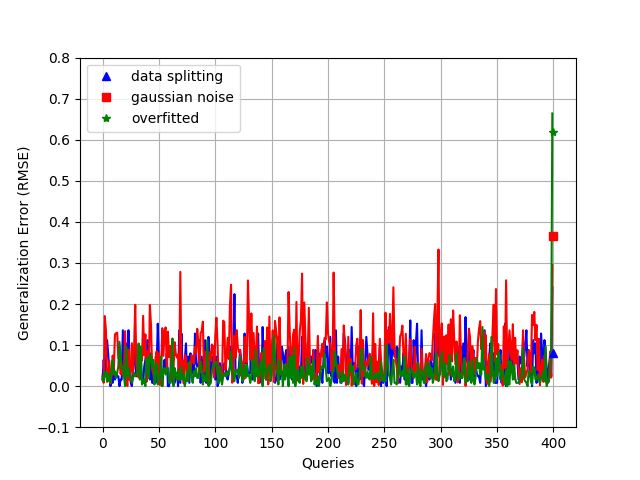
\includegraphics[width=0.9\textwidth]{figures/tworound.png}
\caption{}
\end{centering}
\end{subfigure}
%}
\quad
\begin{subfigure}{.48\textwidth}
\begin{centering}
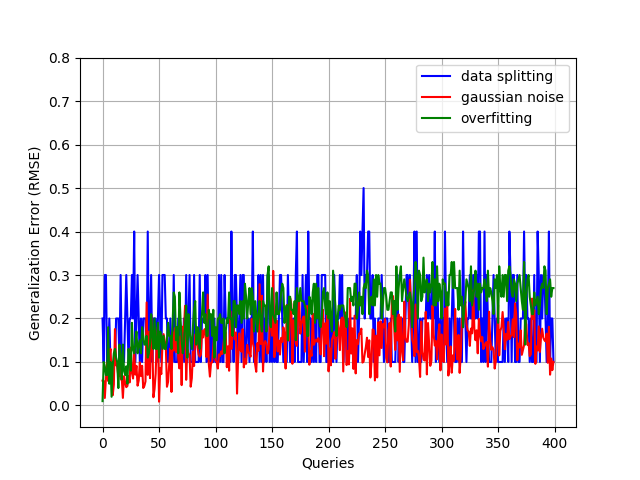
\includegraphics[width=0.9\textwidth]{figures/multipleround.png}
\caption{}
\end{centering}
\end{subfigure}
\vspace{-0.4cm}
 \caption{
 The generalization errors of two adaptive data analysis examples, under different choices of mechanisms.
 (a) Data analysis with adaptivity 2, 
 (b) Data analysis with adaptivity 400. 
}
\label{fig:generalization_errors}
\vspace{-0.5cm}
\end{figure}
}
%gap
This scenario motivates us to explore the design of program analysis techniques that can be used to estimate the number of \emph{rounds of adaptivity} that a program implementing a data analysis can perform. These techniques could be used to help a data analyst in the choice of the mechanism to use,
and they
could ultimately be integrated into a tool for adaptive data analysis such as the \emph{Guess and Check} framework by~\cite{RogersRSSTW20}. 
%